%%%%%%%%%%%%%%%%%%%%%%%%%%%%% Define Article %%%%%%%%%%%%%%%%%%%%%%%%%%%%%%%%%%
\documentclass{article}
%%%%%%%%%%%%%%%%%%%%%%%%%%%%%%%%%%%%%%%%%%%%%%%%%%%%%%%%%%%%%%%%%%%%%%%%%%%%%%%

%%%%%%%%%%%%%%%%%%%%%%%%%%%%% Using Packages %%%%%%%%%%%%%%%%%%%%%%%%%%%%%%%%%%
\usepackage{geometry}
\usepackage{graphicx}
\usepackage{amssymb}
\usepackage{amsmath}
\usepackage{amsthm}
\usepackage{empheq}
\usepackage{mdframed}
\usepackage{booktabs}
\usepackage{lipsum}
\usepackage{graphicx}
\usepackage{color}
\usepackage{psfrag}
\usepackage{pgfplots}
\usepackage{bm}
\usepackage{listings}
\usepackage{tabularx}
\usepackage{array}
\usepackage{subcaption}
%%%%%%%%%%%%%%%%%%%%%%%%%%%%%%%%%%%%%%%%%%%%%%%%%%%%%%%%%%%%%%%%%%%%%%%%%%%%%%%

% Other Settings

%%%%%%%%%%%%%%%%%%%%%%%%%% Page Setting %%%%%%%%%%%%%%%%%%%%%%%%%%%%%%%%%%%%%%%
\geometry{a4paper}

%%%%%%%%%%%%%%%%%%%%%%%%%% Define some useful colors %%%%%%%%%%%%%%%%%%%%%%%%%%
\definecolor{ocre}{RGB}{243,102,25}
\definecolor{mygray}{RGB}{243,243,244}
\definecolor{deepGreen}{RGB}{26,111,0}
\definecolor{shallowGreen}{RGB}{235,255,255}
\definecolor{deepBlue}{RGB}{61,124,222}
\definecolor{shallowBlue}{RGB}{235,249,255}
%%%%%%%%%%%%%%%%%%%%%%%%%%%%%%%%%%%%%%%%%%%%%%%%%%%%%%%%%%%%%%%%%%%%%%%%%%%%%%%

%%%%%%%%%%%%%%%%%%%%%%%%%%%%%%% Listing Settings %%%%%%%%%%%%%%%%%%%%%%%%%%%%%%
\definecolor{codegreen}{rgb}{0,0.6,0}
\definecolor{codegray}{rgb}{0.5,0.5,0.5}
\definecolor{codepurple}{rgb}{0.58,0,0.82}
\definecolor{backcolour}{rgb}{0.95,0.95,0.92}

\lstdefinestyle{mystyle}{
    backgroundcolor=\color{backcolour},   
    commentstyle=\color{codegreen},
    keywordstyle=\color{magenta},
    numberstyle=\tiny\color{codegray},
    stringstyle=\color{codepurple},
    basicstyle=\ttfamily\footnotesize,
    breakatwhitespace=false,         
    breaklines=true,                 
    captionpos=b,                    
    keepspaces=true,                 
    numbers=left,                    
    numbersep=5pt,                  
    showspaces=false,                
    showstringspaces=false,
    showtabs=false,                  
    tabsize=2
}

\lstset{style=mystyle}
%%%%%%%%%%%%%%%%%%%%%%%%%%%%%%%%%%%%%%%%%%%%%%%%%%%%%%%%%%%%%%%%%%%%%%%%%%%%%%%

%%%%%%%%%%%%%%%%%%%%%%%%%% Define an orangebox command %%%%%%%%%%%%%%%%%%%%%%%%
\newcommand\orangebox[1]{\fcolorbox{ocre}{mygray}{\hspace{1em}#1\hspace{1em}}}
%%%%%%%%%%%%%%%%%%%%%%%%%%%%%%%%%%%%%%%%%%%%%%%%%%%%%%%%%%%%%%%%%%%%%%%%%%%%%%%

%%%%%%%%%%%%%%%%%%%%%%%%%%%% English Environments %%%%%%%%%%%%%%%%%%%%%%%%%%%%%
\newtheoremstyle{mytheoremstyle}{3pt}{3pt}{\normalfont}{0cm}{\rmfamily\bfseries}{}{1em}{{\color{black}\thmname{#1}~\thmnumber{#2}}\thmnote{\,--\,#3}}
\newtheoremstyle{myproblemstyle}{3pt}{3pt}{\normalfont}{0cm}{\rmfamily\bfseries}{}{1em}{{\color{black}\thmname{#1}~\thmnumber{#2}}\thmnote{\,--\,#3}}
\theoremstyle{mytheoremstyle}
\newmdtheoremenv[linewidth=1pt,backgroundcolor=shallowGreen,linecolor=deepGreen,leftmargin=0pt,innerleftmargin=20pt,innerrightmargin=20pt,]{theorem}{Theorem}[section]
\theoremstyle{mytheoremstyle}
\newmdtheoremenv[linewidth=1pt,backgroundcolor=shallowBlue,linecolor=deepBlue,leftmargin=0pt,innerleftmargin=20pt,innerrightmargin=20pt,]{definition}{Definition}[section]
\theoremstyle{myproblemstyle}
\newmdtheoremenv[linecolor=black,leftmargin=0pt,innerleftmargin=10pt,innerrightmargin=10pt,]{problem}{Problem}[section]
%%%%%%%%%%%%%%%%%%%%%%%%%%%%%%%%%%%%%%%%%%%%%%%%%%%%%%%%%%%%%%%%%%%%%%%%%%%%%%%

%%%%%%%%%%%%%%%%%%%%%%%%%%%%%%% Plotting Settings %%%%%%%%%%%%%%%%%%%%%%%%%%%%%
\usepgfplotslibrary{colorbrewer}
\pgfplotsset{width=8cm,compat=1.9}
%%%%%%%%%%%%%%%%%%%%%%%%%%%%%%%%%%%%%%%%%%%%%%%%%%%%%%%%%%%%%%%%%%%%%%%%%%%%%%%

%%%%%%%%%%%%%%%%%%%%%%%%%%%%%%% Title & Author %%%%%%%%%%%%%%%%%%%%%%%%%%%%%%%%
\title{Freedom of Press Among World Nations}
\author{Shakleen Ishfar \and Eugene Ayonga}
%%%%%%%%%%%%%%%%%%%%%%%%%%%%%%%%%%%%%%%%%%%%%%%%%%%%%%%%%%%%%%%%%%%%%%%%%%%%%%%

\begin{document}
    \maketitle

    \section{Introduction}

    There are many news organizations around the world. News organizations play a vital role in relaying important news of home and abroad to its readers. These news often cover incidents that are either positive, negative, or neutral. Moreover, some news stories can be viewed as talking for a country or talking against it. 

    Freedom of speech is the right to express ideas and opinions without censorship, restraint, or fear of retribution. A news outlet is free if it can report news in an unbiased manner and free from censorship. In this project, we aim to detect if a local news organization is free. To do so, we compare the sentiment and stance of the organization with international news reporting institutions \textbf{Reuters} and \textbf{Associated Press}. We assume that the more similar a local news is, in terms of sentiment and stance, to the international media outlets, the more free it is. 
    
    In summary, this study investigates freedom of speech in local news across countries, examining topic-specific distinctions by comparing sentiment and stance scores with international sources to reveal distinctions and assess agreement levels.

    \section{Related Work}
    % TODO: Cite similar works

    \section{Methodology}

    The methodlogy of our study can be summarized as follows:

    \begin{enumerate}
        \item \textbf{Data Accumulation}: Select countries to study and collect local-international news articles specific to these countries.
        \item \textbf{Data Processing}: We prepared the data for analysis by performing text processing.
        \item \textbf{Topic Modeling}: To compare relevant news articles from both sources we need to first find the topics and categorize news into these topics.
        \item \textbf{Sentiment and stance analysis}: For each news article, we need to find its sentiment and stance. Specifically, by sentiment, we mean whether a news is positive or neutral or negative. And by stance, we mean whether the news is in support of the local nation or impartial or against it.
        \item \textbf{Hypothesis testing}: Finally, we perform hypothesis testing on the sentiment and stance score for both source of news. This allows us to come to statistically significant conclusions.
    \end{enumerate}

    \subsection{Data Acquisition}

    For this study, we decided to move forward with three countries, Canada, China, and Russia. The countries were picked based on political inclinations. For each of these countries, we collected news from local and international sources. Table \ref{table:data_sources} presents our data sources for each countries.

    \begin{table}[ph]
        \centering
        \begin{tabular}{|c|l|l|l|}
            \hline
            Source Type & Canada & China & Russia \\
            \hline
            Local & Global News & China Daily & The Moscow Times \\
            \hline
            International & \multicolumn{3}{c|}{Reuters and Associated Press} \\
            \hline
        \end{tabular}
        \caption{Data sources for countries under study}
        \label{table:data_sources}
    \end{table}

    We used \emph{Selenium} and \emph{News Please} to collect our news corpus. In particular, we crawled news websites using Selenium and collected articles URLs. Afterwards, we scraped article data using \emph{News Please}. News Please gives us a lot of data about the articles. \cite{Hamborg2017} The following are properties of interest for our study:

    \begin{enumerate}
        \item \textbf{Title}: The title of the articles.
        \item \textbf{Description}: A short description of the article. Typically, the subheading of the article.
        \item \textbf{Maintext}: The body of the article.
        \item \textbf{Publication Date}: When the article was published.
    \end{enumerate}

    Our accumulated data and their countrywise distribution is shown in figure \ref{fig:raw_data}.
    
    \begin{figure}[ht]
        \centering
        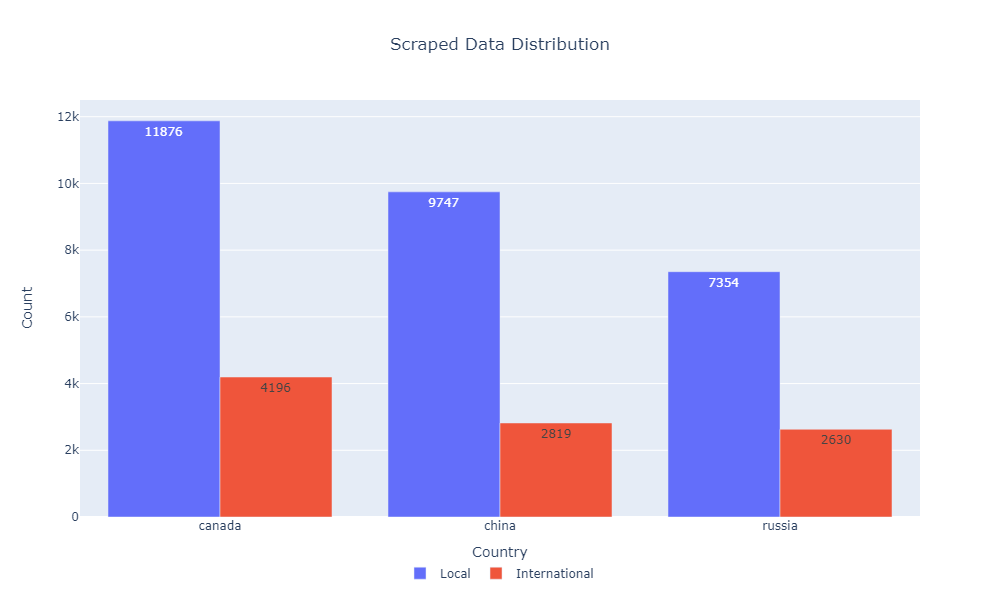
\includegraphics[width=0.75\linewidth]{../images/plots/barchart_scraped_data.png}
        \caption{Collected data across countries of interest from local and international sources}
        \label{fig:raw_data}
    \end{figure}

    \subsection{Data Processing}

    To prepare the data for topic modeling and sentiment-stance analysis we had to process the dataset. This inlcludes the following:

    \begin{enumerate}
        \item \textbf{Imputation}: Many of the URLs scraped by News Please, some attributes were null. The first step was filling in those values. We chose to replace null text columns with empty strings.
        \item \textbf{Duplicate removal}: In this step, we detected duplicate article data and removed them. In particular, we detected duplicates by comparies the \emph{publication data} and \emph{title} attributes.
        \item \textbf{Text level processing} \begin{itemize}
            \item Remove HTML tags, links, emails, phone numbers, etc.
            \item Discard editorial information, e.g. "Published by Global News".
            \item Strip non-ASCII characters.
            \item Remove editorial information, e.g. written by X, photo by Y, etc.
        \end{itemize}
        \item \textbf{Row level processing} \begin{itemize}
            \item Drop rows with empty titles and maintext.
            \item Filter out unrelated geographical news.
            \item Remove rows where the maintext is too short.
        \end{itemize}
        \item \textbf{Country level processing} \begin{itemize}
            \item Global news in particular reports inflation news. This sort of articles don't have a lot of text and is strictly tabular. We decided not to include this sort of news in our analysis.
            \item Removed Israel-Palestine from all country news corpus. As they are not relevant to the countries being studied.
        \end{itemize}
    \end{enumerate}

    \subsection{Topic Modeling}

    BERTopic is an unsupervised machine Learning  algorithm for topic modeling. It leverages Bidirectional Encoder Representations from Transformers (BERT) and c-TF-IDF (Class-Based Term Frequency - Inverse Document Frequency) to create coherent and easily interpretable topics, described by automatically generated labels. It has a number of sub-components, which are discussed below, whose understanding at a higher level can inherently improve the topic modeling performance. \cite{grootendorst2022bertopic}
    
    \begin{figure}[ht]
        \centering
        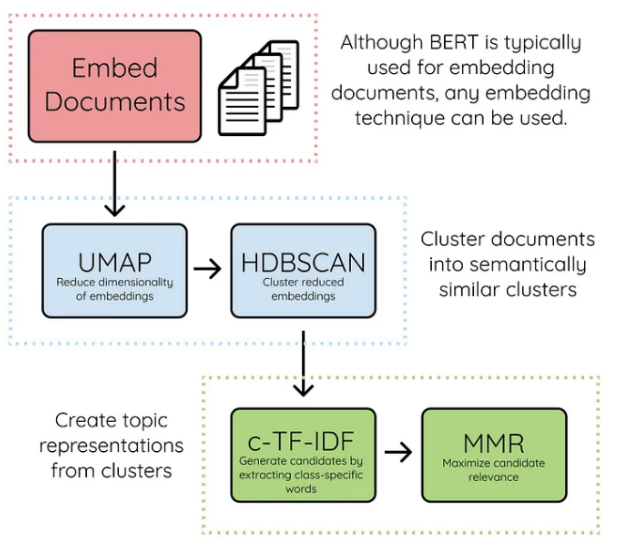
\includegraphics[width=0.5\linewidth]{../images/BERTopic_diagram.png}
        \caption{BERTopic Diagram}
        \label{fig:bertopic_diagram}
    \end{figure}

    \subsubsection{Transformer Embedding Model}
    The model embeds Input documents to sentence vector representations which are typically dense in nature. In this project, we used sentence transformers to capture semantic similarity, as it provides an extensive library of high performing sentence embeddings. The L6-v2 version created 384-dimensional sentence embeddings.

    \subsubsection{Dimensionality Reduction}
    As a next step, BERTopic then performs dimensionality reduction of the 384-dimension sentence embeddings into a lower-dimensional space, either two or three-dimensional vectors. This project used the BERTopic default; Uniform Manifold Approximation and Projection (UMAP). UMAP captures both the local and global high-dimensional space in lower dimensions.

    Since BERTopic provides room for independence between steps, other popular choices for dimensionality reduction such as Principal Components Analysis (PCA) and t-distributed Stochastic Neighbour Embedding (t-SNE) can be used.

    PCA works by preserving larger distances by mean squared error. This results in the data's global structure being reserved; a pro when there are clusters that are easily distinguishable in the dataset. A demerit of using PCA is that it falls short when dealing with more nuanced data where local structures are vital. Inversely, t-SNE main characteristic is the preservation of similarity. UMAP exploits the best of both worlds, thus an appropriate technique.

    \subsubsection{Clustering}

    Involves clustering dimensionally reduced embeddings into groups of similar embeddings to extract topics. There are an array of clustering techniques such as partition-based, hierarchical based and density-based, to name but a few. Each one of them has its own advantages and disadvantages.

    Hierarchical Density Based Spatial Clustering of Applications with Noise (HDBSCAN) is both hierarchical and density-based. It is BERTopic's default that is typically used to capture structures with different densities. Advantages of HDBSCAN include: ease of tuning and visualizing hierarchical data, outlier identification and the ability to cluster irregular shapes. 

    Since BERTopic's independence between steps still hold, K-means can be used for clustering using a centroid approach. A drawback would be poor handling of noisy clusters.

    \subsubsection{Vectorizers}

    As a final step of the BERTopic workflow, topic extraction from the clusters formed in the previous step is done. BERTopic applies the use of a modified version of TF-IDF called Class-Based Term Frequency – Inverse Document Frequency (c-TF-IDF), which finds the most essential and relevant terms given to each document within a cluster. A CountVectorizer is initialized, and together with TF-IDF, topic representations are created, allowing for parameter fine tuning.

    \begin{figure}[hp]

        \centering
        \begin{subfigure}{0.45\textwidth}
            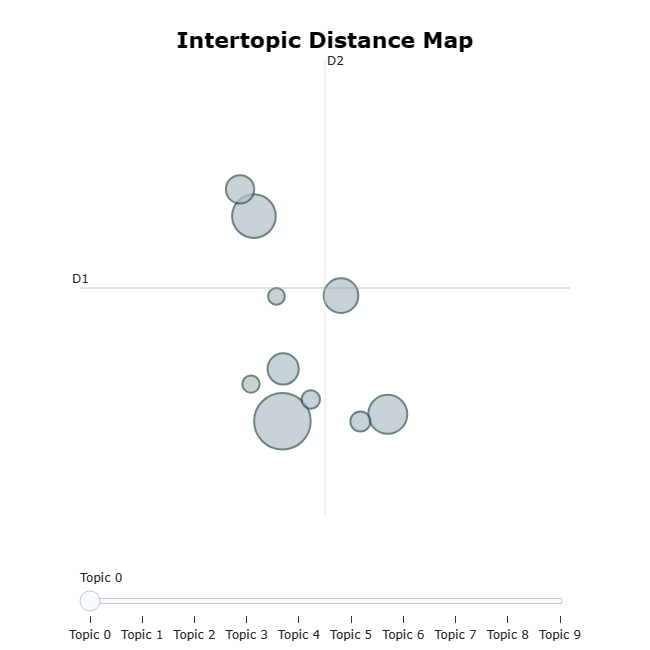
\includegraphics[width=\textwidth]{../images/plots/Canada/intertopic_distance_map_canada.png}
            \caption{Canada Intertopic Map}
            \label{fig:intertopic_canada}
        \end{subfigure}
        \hfill
        \begin{subfigure}{0.45\textwidth}
            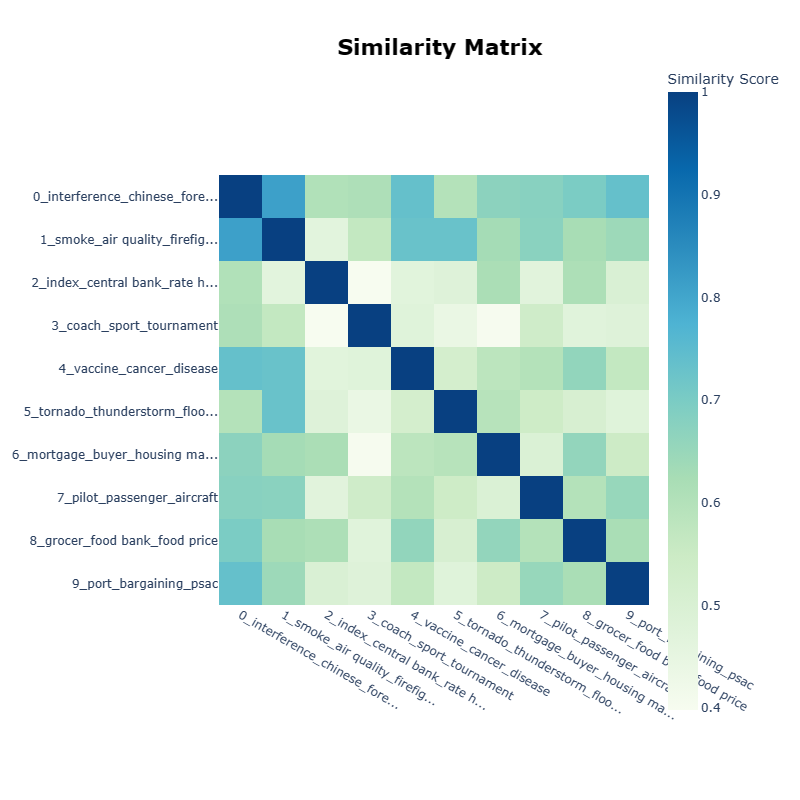
\includegraphics[width=\textwidth]{../images/plots/Canada/similarity_matrix_canada.png}
            \caption{Canada Similarity Matrix}
            \label{fig:sim_canada}
        \end{subfigure}
        \hfill
        
        \begin{subfigure}{0.45\textwidth}
            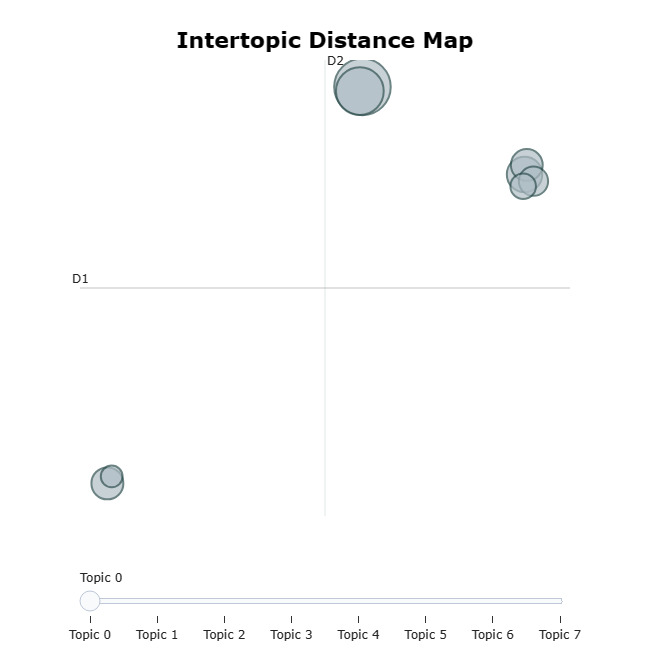
\includegraphics[width=\textwidth]{../images/plots/China/intertopic_distance_map_china.png}
            \caption{China Intertopic Map}
            \label{fig:intertopic_china}
        \end{subfigure}
        \hfill
        \begin{subfigure}{0.45\textwidth}
            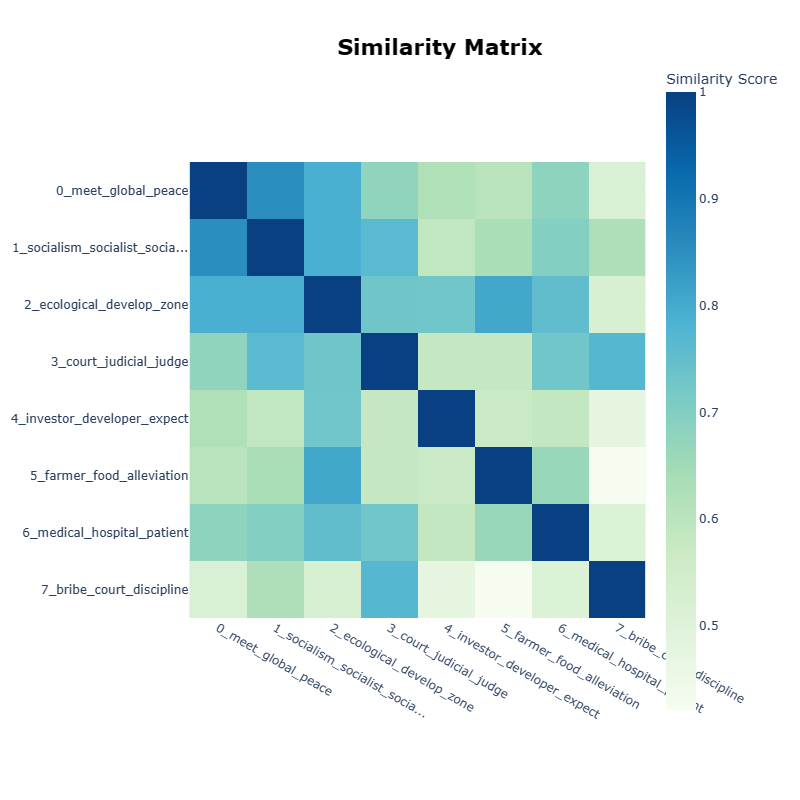
\includegraphics[width=\textwidth]{../images/plots/China/similarity_matrix_china.png}
            \caption{China Similarity Matrix}
            \label{fig:sim_china}
        \end{subfigure}
        \hfill

        \begin{subfigure}{0.45\textwidth}
            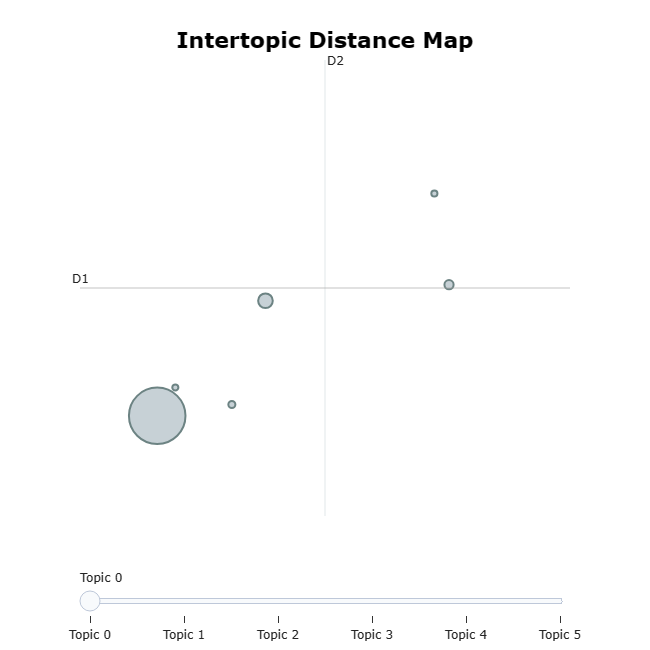
\includegraphics[width=\textwidth]{../images/plots/Russia/intertopic_distance_map_russia.png}
            \caption{Russia Intertopic Map}
            \label{fig:intertopic_russia}
        \end{subfigure}
        \hfill
        \begin{subfigure}{0.45\textwidth}
            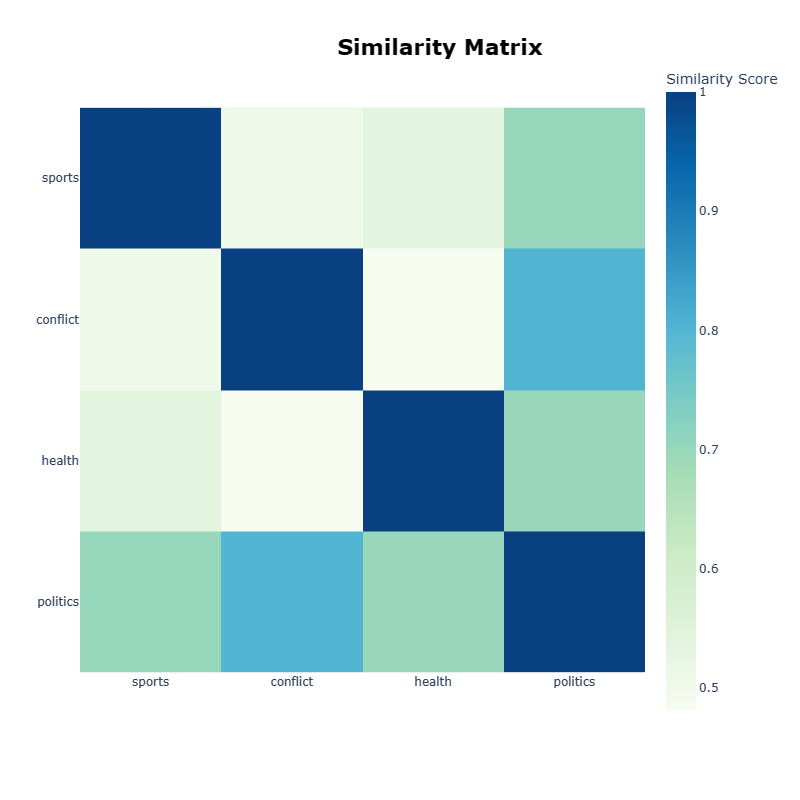
\includegraphics[width=\textwidth]{../images/plots/Russia/similarity_matrix_russia.png}
            \caption{Russia Similarity Matrix}
            \label{fig:sim_russia}
        \end{subfigure}
                
        \caption{Intertopic distance maps and similarity matrices for accessing quality of topic models}
        \label{fig:topic_model_quality}
    \end{figure}

    \subsubsection{Topic Quality}
    After tuning the different parameters, we were able to generate topics for our collected data. Figure \ref{fig:topic_model_quality} shows the quality of the topic models. A good topic model will have topics that have low intertopic similarity. Moreover, the bubbles in the intertopic distance map should be large and non-overlapping. The figures clearly show this for our modeled topics. Here are a few interesting observations:

    \begin{enumerate}
        \item Canadian news has the most amount of topics. Moreover, most of the topics seem to be quite dissimilar to one another.
        \item Chinese news topics have more similarity between topics. But the media covers a wide array of topics in general.
        \item Russian news media seem to cover more political news. This is expected as there is a war that's ongoing.
    \end{enumerate}

    \subsection{Sentiment and Stance Analysis}

    For sentiment and stance analysis, we decided to use a Large Language Model (LLM). 
    
    \subsubsection{Utilization of LLM}
    LLMs are excellent for natural language understanding and generation tasks. \cite{boiko2023emergent} We used these capabilities of an LLM in the following way:

    \begin{enumerate}
        \item \textbf{Classification}: Classify the document's sentiment as positive or negative or neutral. Classify the stance as for or neutral or against the local country.
        \item \textbf{Scoring}: Assign a score from -1.0 (negative / against) to +1.0 (positive / for) for sentiment and stance.
        \item \textbf{Reason}: The LLM gives a short one sentence reason behind its classification and scoring.
    \end{enumerate}

    We decided to use the open-source \textbf{LLaMa-2} model, from \emph{Meta}. For our training and inference pipeline we heavily relied on \emph{HuggingFace}. \cite{touvron2023llama}

    \subsubsection{Finetune LLaMa-2}

    To finetune our model, we select 300 samples randomly. 100 samples for each country, and 50 samples for each source type. Afterwards, we engineered an effective prompt using \emph{Prompt Perfect} for LLaMa-2. The prompt is shown in listing \ref{listing:prompt_llama}. It should be noted that we replaced \emph{\{title\}} and \emph{\{content\}} with the actual title and content of the news article being analyzed.

    \begin{lstlisting}[caption=Prompt for LLaMa, label={listing:prompt_llama}]
As a neutral news analyst, assess the sentiment and stance of the news article
excerpt and assign a score between -1.0 (completely negative/against-{country}) 
and 1.0 (completely positive/pro-{country}) for both sentiment and stance. 
Provide a single short sentence to justify your scores, drawing on the article's
language, tone, and presentation to support your analysis.

Article Excerpt:
- Title: "{title}"
- Content: "{content}"

Output format: 
1. Sentiment: [Positive/Neutral/Negative]
    * Score: [Your Score]
    * Reason: [Your Reason] 
2. Stance: [Pro-{country}/Impartial/Against-{country}]
    * Score: [Your Score]
    * Reason: [Your Reason]
    \end{lstlisting}
    
    To create the finetuning dataset, we fed the 300 articles into ChatGPT using the prompt structure shown above. Next, we finetuned the base model from HuggingFace user \emph{TinyPixel} in the following way:

    \begin{itemize}
        \item \textbf{Sharded Base model}: A sharded base model allowed us to load chunks of the model one at a time. This, along with QLoRA, allowed us to train the model on a single GPU in google colab.
        \item \textbf{QLoRA}: We used QLoRA to quantize the model and train a 4-bit version of the LLM. Simply, this allows us to train a subset of the model's parameters instead of the entire model. This allowed us to finetune the model with only a single GPU. \cite{dettmers2023qlora}
        \item \textbf{PEFT}: Parameter Efficient Fine Tuning was used to train a subset of the model's parameters instead of the entire model. This allowed us to train the model quickly while retaining high performance.
    \end{itemize}

    After finetuning the model, 4000 samples were selected for each country. Then the sentiment and stance of those countries were predicted using LLaMa-2.

    \subsection{Hypothesis Testing}
    After getting the scores for our dataset, we performed statistical analysis on the scores of the news. In particular, we performed the following hypothesis tests:

    \begin{table}[hp]
        \centering
        \begin{tabular}{ | m{2cm} | m{3cm}| m{8cm} | } 
          \hline
          \textbf{Test} & \textbf{Parameter of Interest} & \textbf{The Question We Ask} \\ 
          \hline
            Welch Test & Mean & Does the average score from both sources have any difference? \\
            \hline
            Wilcoxon Test & Median & Is the meidan score from sources different? \\
            \hline
            Variance Test & Varaince & Does the content from both sources cover a similar range of sentiment or stance? \\
            \hline
            Pearson's Test & Correlation & Is there any linear correlation between the scores from both sources? \\
            \hline
            Spearman's Test & Monotonic Relation & Is there any monotonic relationship between the scores from both sources? \\
            \hline
        \end{tabular}

        \caption[Prompt Engineering]{Role and Goal prompt engineering and output}
        \label{table:prompt_engineering}
    \end{table}

    All tests were done with a confidence level of 99\%. Since we have a lot of data, we wanted to be sure to come to a conclusion. 

    \section{Experiment}
    
    We break our expriment into 3 case studies. Each case study covers a specific country and analyzes the news from both local and international sources.

    \subsection{Canada}
    From figure \ref{fig:canada_topic}, we can see than Canadian news covers a wide range of topics.
    
    \begin{figure}[hp]
        \centering
        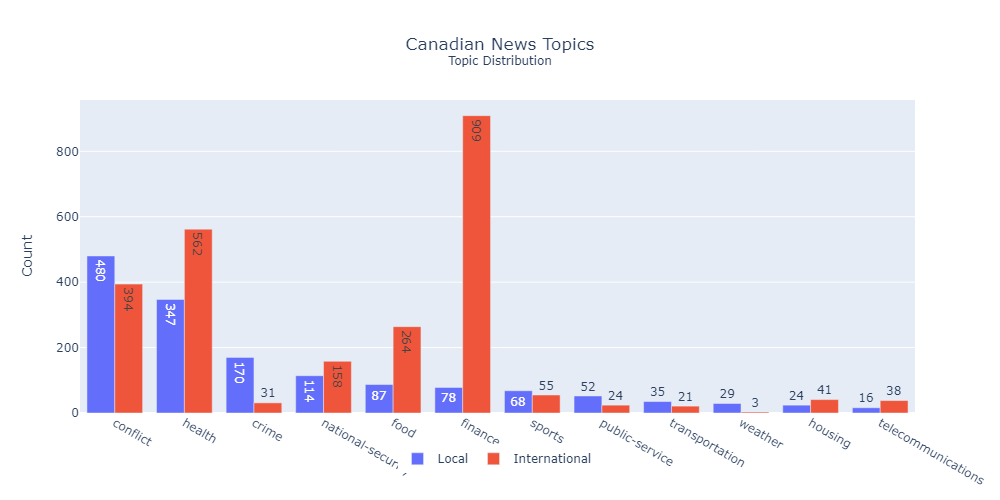
\includegraphics[width=\linewidth]{../images/plots/Canada/canada_barchart_topics.png}
        \caption{Canadian news topics bar chart.}
        \label{fig:canada_topic}
    \end{figure}

    \subsubsection{Sentiment Analysis}

    We first begin by showing the distribution of the sentiment scores for each topic from both the local and international media in figure \ref{fig:canada_sentiment_score_boxplot}. 
    
    \begin{figure}[hp]
        \centering
        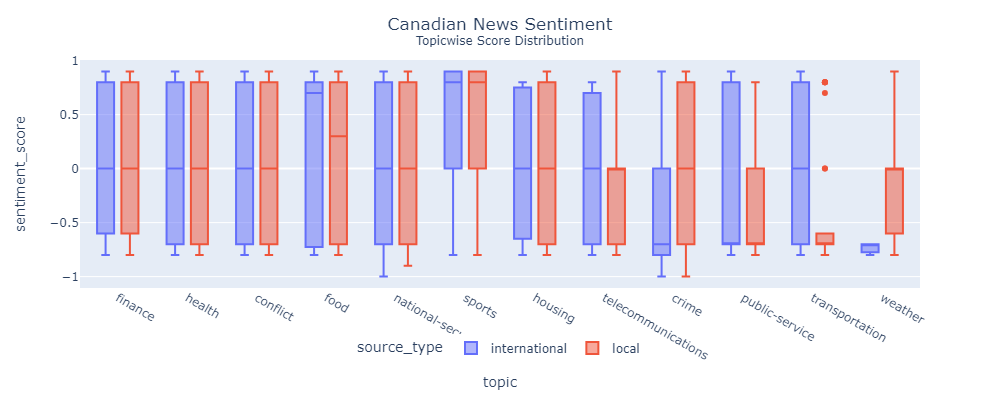
\includegraphics[width=\linewidth]{../images/plots/Canada/canada_boxplot_sentiment.png}
        \caption{Boxplot showing the topicwise distribution of canadian news sentiment scores for local and international media outlets.}
        \label{fig:canada_sentiment_score_boxplot}
    \end{figure}

    Some distinctions are clearly visible here. For example:

    \begin{itemize}
        \item \emph{Sports} news from both sources tends to have a positive sentiment. Both sources seem to have the same sentiment in this topic.
        \item \emph{Telecommunication} news from international media seem to cover a wide spectrum of sentiment while local media seem to convey a more negative portrayal of the matter. \emph{Public-service} has the same distribution while \emph{Crime} has the opposite.
        \item \emph{Transportation} and \emph{weather} has a noticable distinction in their score distribution for both sources.
    \end{itemize}

    We run statistical inference tests to find these distinctions mathematically. The results are shown in figure \ref{fig:canada_sentiment_score_heatmap}.

    \begin{figure}[hp]
        \centering
        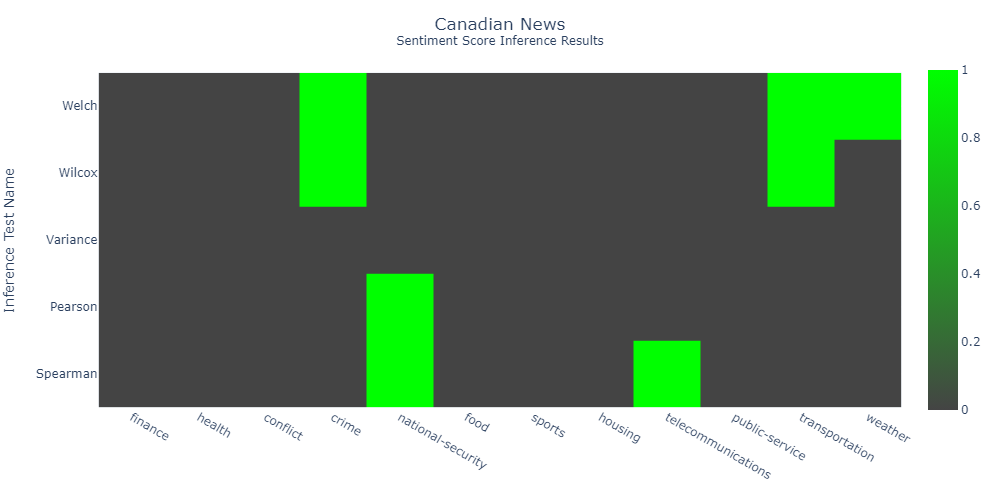
\includegraphics[width=\linewidth]{../images/plots/Canada/canada_heatmap_inference_sentiment.png}
        \caption{Heatmap showing the result of topicwise inference tests done on canadian news sentiment scores.}
        \label{fig:canada_sentiment_score_heatmap}
    \end{figure}

    \begin{itemize}
        \item \emph{Crime}, \emph{transportation}, and \emph{weather} is statistically significant in terms of Welch and Wilcoxon test. Which means that on average the sentiment scores from both sources are different. This means both sources typically report news that are of different sentiment.
        \item \emph{National-security} is statistically significant in terms of Pearson's and Spearman's test. Which means the score of the two sources aren't independent of each other. There exists some sort of a correlation or monotonic relationship. This means that the two sources report news that are somewhat related. 
    \end{itemize}

    \subsubsection{Stance Analysis}

    Now let's analyze the stance scores from figure \ref{fig:canada_stance_score_boxplot}. The most interesting observation here is that, international media, in most topics, seem to have an impartial stance, While local news outlet has a more pro-canada stance. The obvious exceptions are \emph{Health} and \emph{Food}.
    
    \begin{figure}[hp]
        \centering
        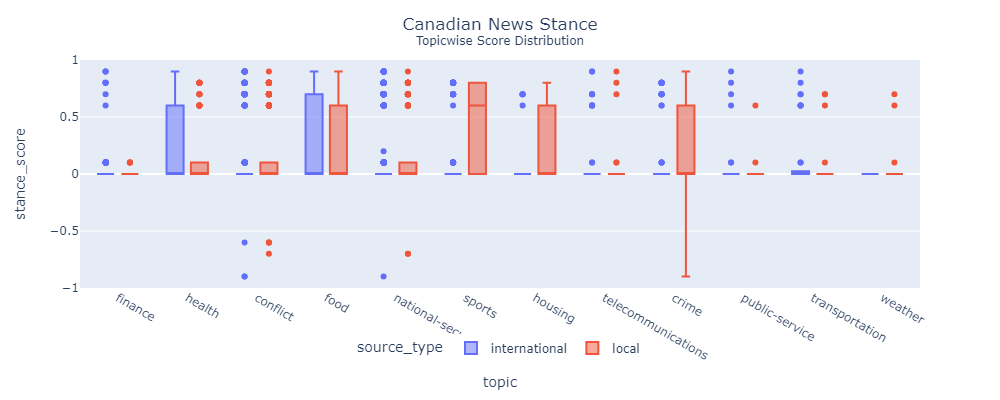
\includegraphics[width=\linewidth]{../images/plots/Canada/canada_boxplot_stance.png}
        \caption{Boxplot showing the topicwise distribution of canadian news stance scores for local and international media outlets.}
        \label{fig:canada_stance_score_boxplot}
    \end{figure}

    From the statistical test results shown in \ref{fig:canada_stance_score_heatmap}, we see a similar result as the sentiment score inference results. 

    \begin{figure}[hp]
        \centering
        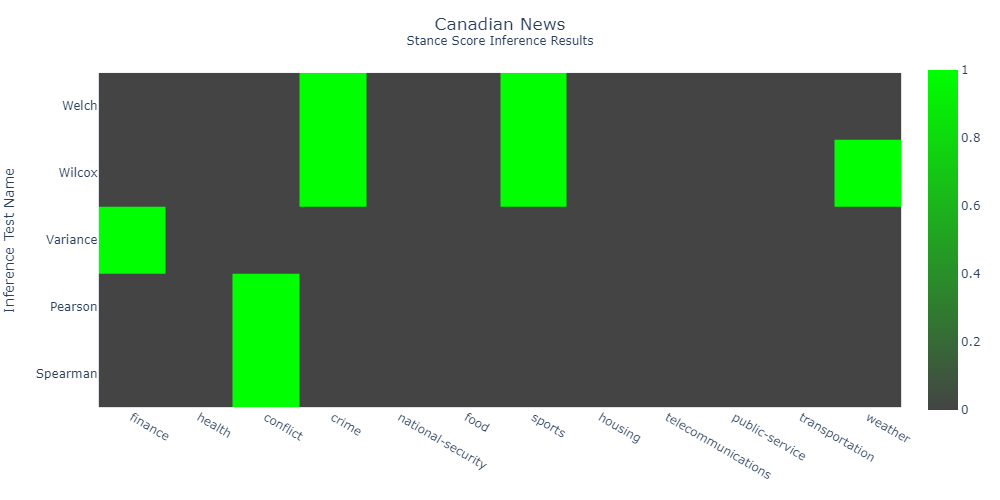
\includegraphics[width=\linewidth]{../images/plots/Canada/canada_heatmap_inference_stance.png}
        \caption{Heatmap showing the result of topicwise inference tests done on canadian news stance scores.}
        \label{fig:canada_stance_score_heatmap}
    \end{figure}
    
    \begin{itemize}
        \item \emph{Crime} and \emph{Sport} relatd news seem to have different stance scores on average.
        \item While \emph{Conflict} related news isn't independent according to Pearson's and Spearman's test.
        \item Interestingly, \emph{Finance} news has a different variance for stance scores. This means, the two sources cover a different range of stances.
    \end{itemize}

    \subsubsection{Text Analysis}

    Let's look at a wordcloud for \emph{Crime} related news from both sources in figure \ref{fig:canada_sentiment_score_wordcloud}.

    \begin{figure}[hp]
        \centering
        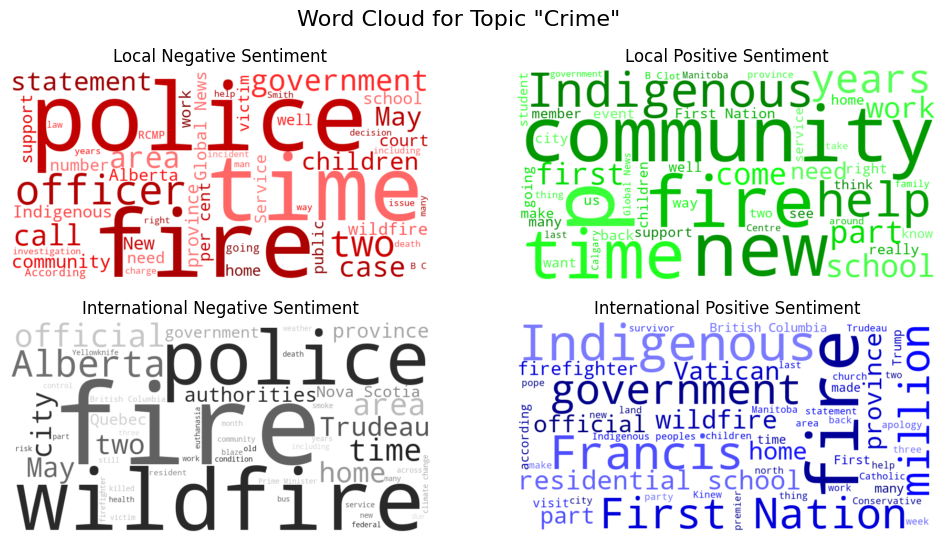
\includegraphics[width=\linewidth]{../images/plots/Canada/canada_wordcloud_crime.png}
        \caption{Word cloud for canadian news about crime.}
        \label{fig:canada_sentiment_score_wordcloud}
    \end{figure}

    We can see that local and international media use the same sort of words across their negative and positive sentiment news. For example, the word police, fire, government appears in the negative sentiment word cloud for both sources. On the other hand, indigenous community, first, fire, etc. are common in the positive sentiment.

    \subsubsection{Verdict}

    Although there is statistically significant distinctions in sentiment for a few topics, both sources report news that are similar in sentiment and stance. Which is why, we find canadian news organization "Global News" as a free press organization.
    
    \subsection{China}

    Let us now look at Chinese news media outlet. Figure \ref{fig:china_topic} shows the distribution of news amongst different topics from both sources. It's clear that both sources publish more news about \emph{politics} than any other topic. The international media also publishes more news about \emph{finance} and \emph{international-relations} than the local news media as well. However, \emph{agriculture} related news is covered mostly by local news outlet.
    
    \begin{figure}[hp]
        \centering
        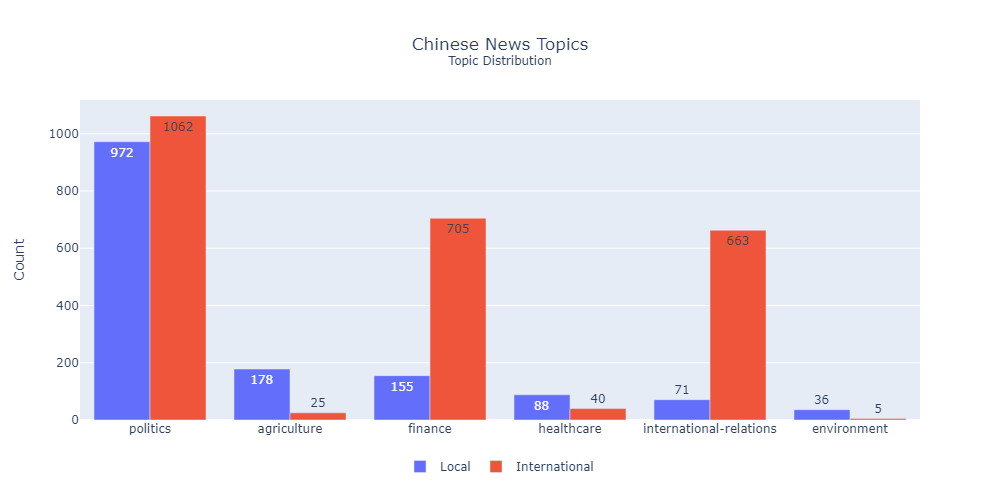
\includegraphics[width=\linewidth]{../images/plots/China/china_barchart_topics.png}
        \caption{Chinese news topics bar chart.}
        \label{fig:china_topic}
    \end{figure}

    \subsubsection{Sentiment Analysis}

    Figure \ref{fig:china_sentiment_score_boxplot} shows the distribution of sentiment scores for various topics for local and international media. 
    
    \begin{figure}[hp]
        \centering
        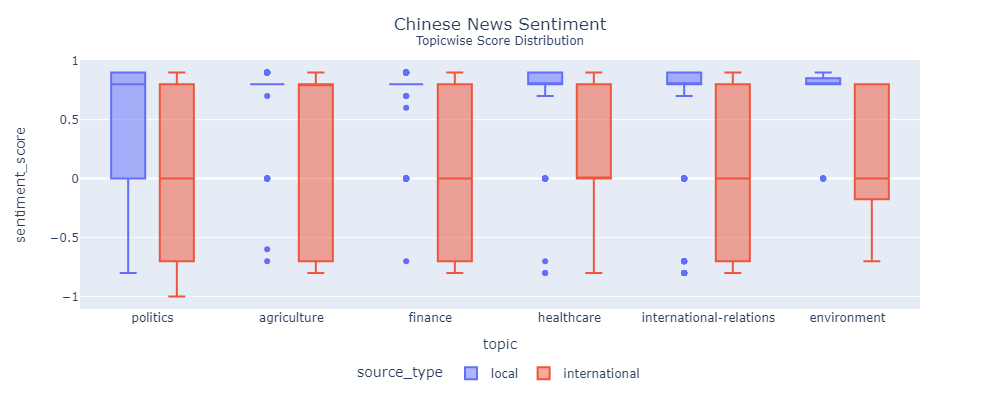
\includegraphics[width=\linewidth]{../images/plots/China/china_boxplot_sentiment.png}
        \caption{Boxplot showing the topicwise distribution of chinese news sentiment scores for local and international media outlets.}
        \label{fig:china_sentiment_score_boxplot}
    \end{figure}  

    One of the most interesting observation is that, the local media in most cases always seems to cover positive sentiment news. Except for a few outliers, their distribution is concentrated towards positive scores. On the other hand, international news covers a wide spectrum of sentiment. 

    \begin{figure}[hp]
        \centering
        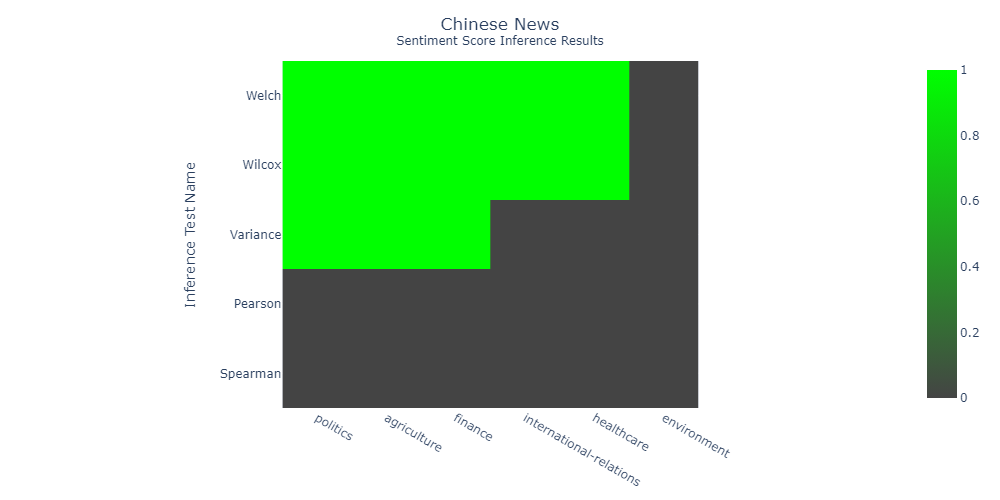
\includegraphics[width=\linewidth]{../images/plots/China/china_heatmap_inference_sentiment.png}
        \caption{Heatmap showing the result of topicwise inference tests done on chinese news sentiment scores.}
        \label{fig:china_sentiment_score_heatmap}
    \end{figure}

    Figure \ref{fig:china_sentiment_score_heatmap} confirms the distinction we saw in the sentiment score distribution. Not only does most topic have on average a different sentiment score, they also have a very different score variance as well. Safe to say that the local and international media cover very different set of news when it comes to sentiment.
    
    \subsubsection{Stance Analysis}    

    From figure \ref{fig:china_stance_score_boxplot}, we observe a similar trend. Local news seem to trend towards pro-china stance while international media is mostly impartial, except for a few outliers. However, local news media seem to cover a few against china news when it comes to \emph{politics} and \emph{international-relations}. On the other hand, \emph{environment} is covered in an impartial to slightly more against-china stance by the international news media.
    
    \begin{figure}[hp]
        \centering
        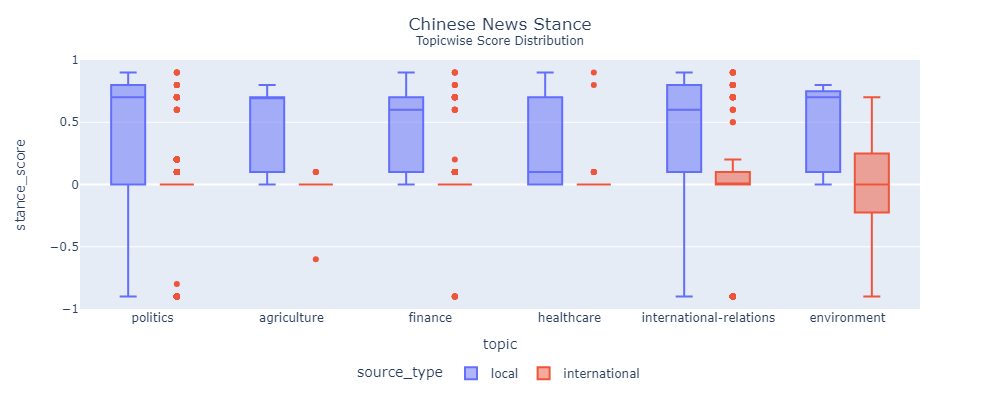
\includegraphics[width=\linewidth]{../images/plots/China/china_boxplot_stance.png}
        \caption{Boxplot showing the topicwise distribution of chinese news stance scores for local and international media outlets.}
        \label{fig:china_stance_score_boxplot}
    \end{figure}

    \begin{figure}[hp]
        \centering
        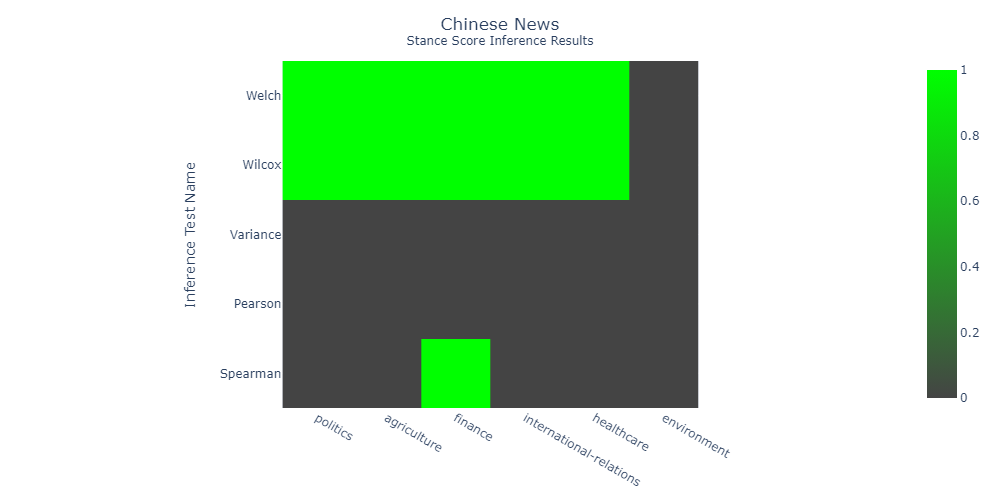
\includegraphics[width=\linewidth]{../images/plots/China/china_heatmap_inference_stance.png}
        \caption{Heatmap showing the result of topicwise inference tests done on chinese news stance scores.}
        \label{fig:china_stance_score_heatmap}
    \end{figure}

    Our observations are confirmed when we see the hypothesis tests results in figure \ref{fig:china_stance_score_heatmap}. Most of the topics, except for \emph{enviornment}, have a statistically significant difference in stance scores. The only reason we don't have a statistically significant difference is that we don't have enough data for this topic. We can also see than most topics are also independent as they are not significant in terms of pearson's and spearman's correlation.

    \subsubsection{Text Analysis}

    \begin{figure}[hp]
        \centering
        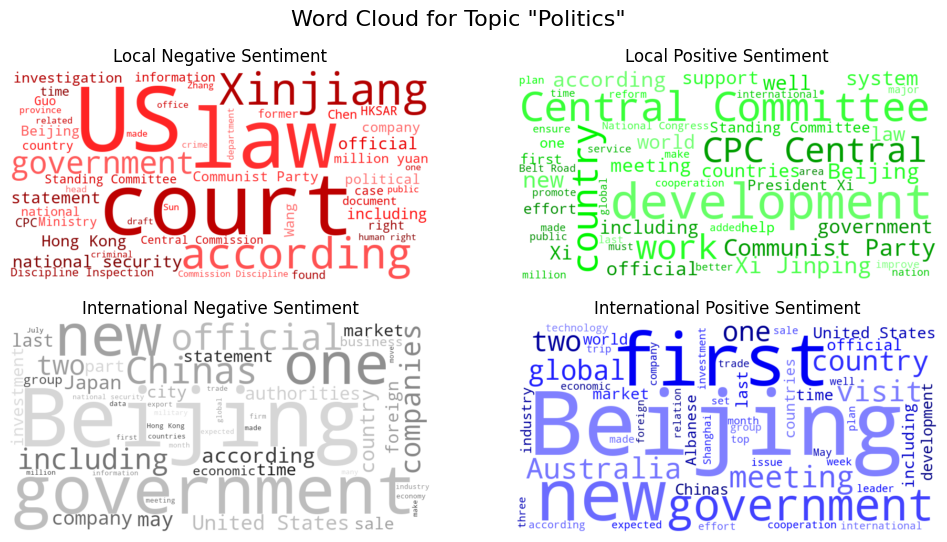
\includegraphics[width=\linewidth]{../images/plots/China/china_wordcloud_politics.png}
        \caption{Word cloud for chinese news about politics.}
        \label{fig:chinese_sentiment_score_wordcloud}
    \end{figure}

    The word cloud for \emph{politics} is shown in figure \ref{fig:chinese_sentiment_score_wordcloud}. Unlike the wordcloud for canadian news, there are less things in common here. For example, in international news, \emph{Beijing}, \emph{government}, and \emph{official} is highlighted in the negative news. While for local news, \emph{US}, \emph{law}, and \emph{court} are highlighted more in the negative sentiment news. International media also talks a lot about \emph{Beijing} and \emph{government} in positive light as well. But the local media seems to talk about \emph{CPC} and \emph{Central Committee} more. Interesting to see that the local media barely has any mention of \emph{Beijing} when the international media is talking about it so much.

    \subsubsection{Verdict}

    There seem to be a lot of dissimilarity when it comes to local news media outlet, "China Daily", and the international news media outlets. Statistically significant differences can be found across most topics. Which is why, we fail to say "China Daily" has freedom of press based on the news samples we have collected.

    \subsection{Russia}

    Finally, we analyze russian news. Figure \ref{fig:russia_topic} shows the distribution of news covered by both local and international media outlets. An interesting observation is that both sources publish more news about \emph{politics} than all other topics combined. Moreover, local news covers more about \emph{health} related news, while international news dives more into the ongoing \emph{conflict} news.
    
    \begin{figure}[hp]
        \centering
        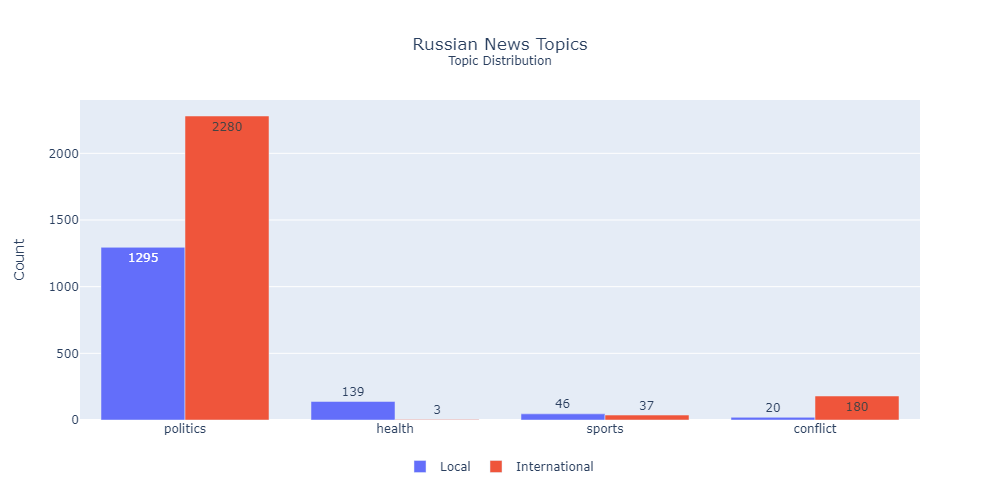
\includegraphics[width=\linewidth]{../images/plots/Russia/russia_barchart_topics.png}
        \caption{Russian news topics bar chart.}
        \label{fig:russia_topic}
    \end{figure}

    \subsubsection{Sentiment Analysis}
    
    \begin{figure}[hp]
        \centering
        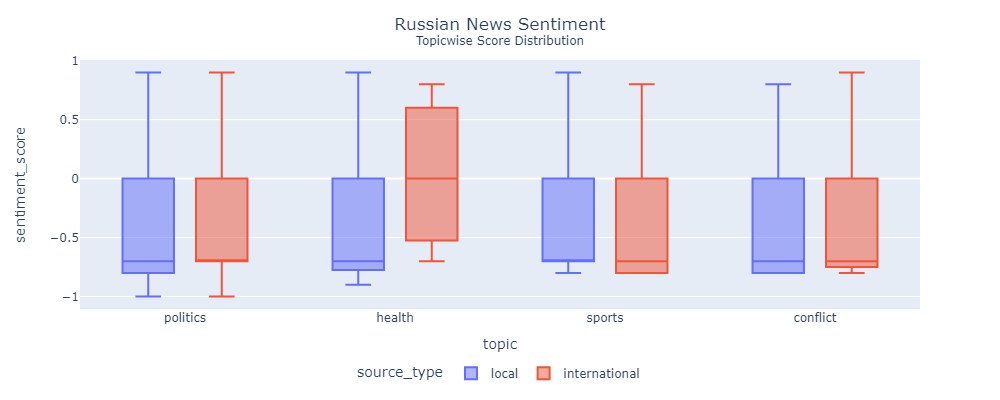
\includegraphics[width=\linewidth]{../images/plots/Russia/russia_boxplot_sentiment.png}
        \caption{Boxplot showing the topicwise distribution of russian news sentiment scores for local and international media outlets.}
        \label{fig:russia_sentiment_score_boxplot}
    \end{figure}  

    From figure \ref{fig:russia_sentiment_score_boxplot} we can see that, unlike chinese news, there are less distinctions in the distribution of the news articles from both sources. \emph{Health} related news seems to be more negative in local media, while the international media is more neutrally distributed. Both new media organizations seem to convey a similar negative sentiment when it comes to \emph{conflict} and \emph{politics}.

    \begin{figure}[hp]
        \centering
        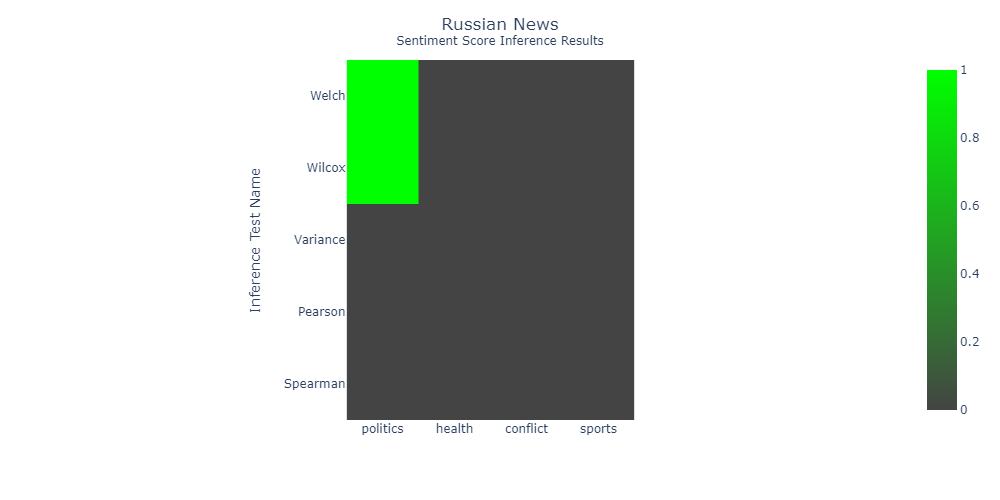
\includegraphics[width=\linewidth]{../images/plots/Russia/russia_heatmap_inference_sentiment.png}
        \caption{Heatmap showing the result of topicwise inference tests done on russian news sentiment scores.}
        \label{fig:russia_sentiment_score_heatmap}
    \end{figure}

    A more interesting observation comes from the statistical test as graphed in figure \ref{fig:russia_sentiment_score_heatmap}. There seems to be a statistically significant difference on the average and median sentiment score between the two sources. 

    \subsubsection{Stance Analysis}
    
    \begin{figure}[hp]
        \centering
        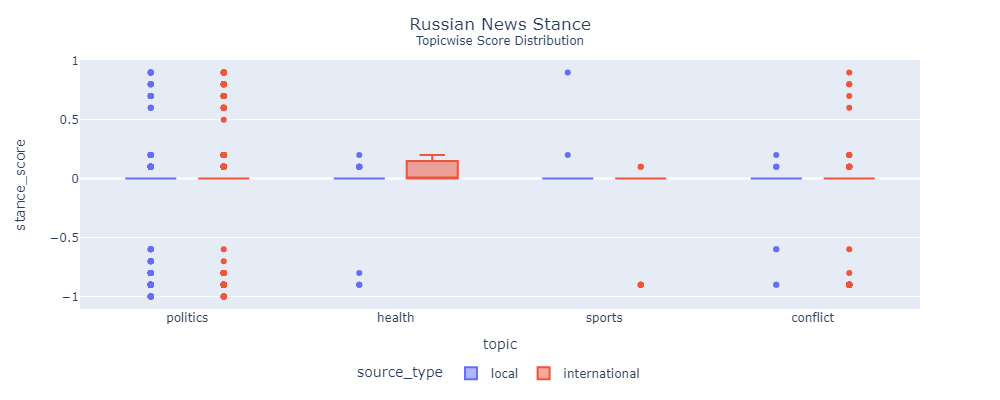
\includegraphics[width=\linewidth]{../images/plots/Russia/russia_boxplot_stance.png}
        \caption{Boxplot showing the topicwise distribution of russian news stance scores for local and international media outlets.}
        \label{fig:russia_stance_score_boxplot}
    \end{figure} 

    The stance scores for both sources seem to be mostly impartial. Except for \emph{Health} related news, where the international media seems to be trendly slightly towards a pro-russian stance.

    \begin{figure}[hp]
        \centering
        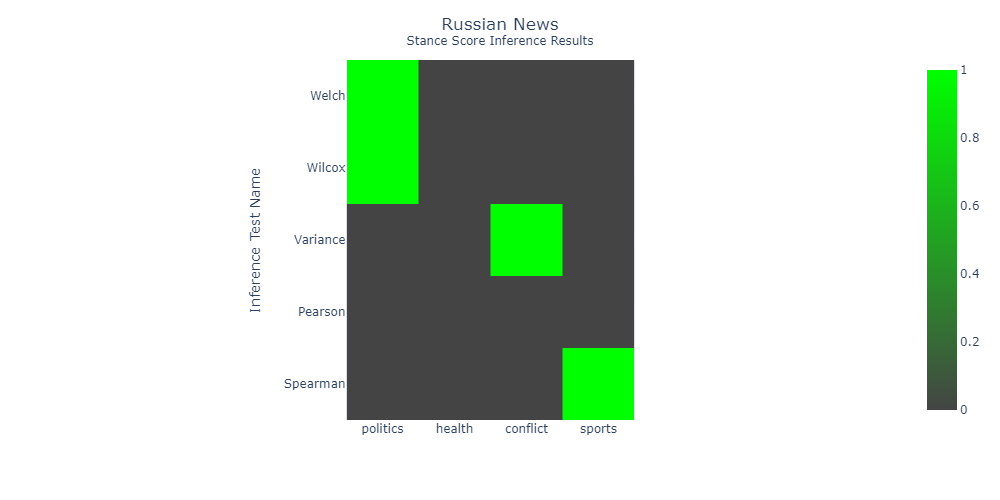
\includegraphics[width=\linewidth]{../images/plots/Russia/russia_heatmap_inference_stance.png}
        \caption{Heatmap showing the result of topicwise inference tests done on russian news stance scores.}
        \label{fig:russia_stance_score_heatmap}
    \end{figure}

    The inference tests for stance, tells the same story as that of the sentiment. Political news on average has different stances from both sources. Interestingly, \emph{conflict} related news has a statistically significant difference in variance. Meaning, local and international news doesn't cover the same range of stance when it comes to this topic. Also, \emph{sports} news has a monotonic relationship between the two sources.

    \subsubsection{Text Analysis}

    Analyzing the word clouds shown in figure \ref{fig:russian_sentiment_score_wordcloud}, we can see that \emph{Ukrain} is a huge talking point across all sentiments regardless of the source. \emph{Putin} also comes up more in local news while \emph{United States} and \emph{China} comes up a lot in international news. In particular, the US seems to be associated more with negative sentiment while China is associated with more positive sentiment. This could indicate the alliance Russia has with China and the animosity it has with the US. Overall, the distinctions in textual content isn't quite as clear as with chinese news.

    \begin{figure}[hp]
        \centering
        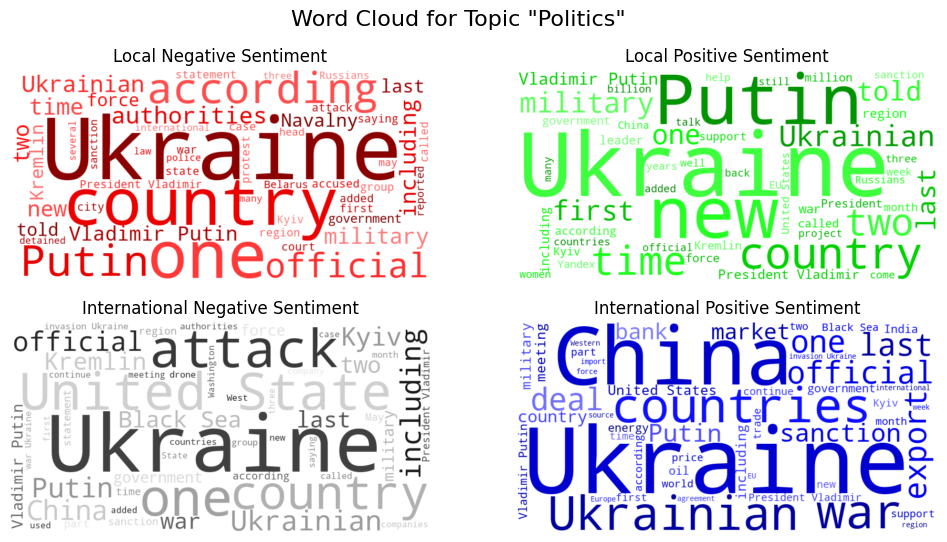
\includegraphics[width=\linewidth]{../images/plots/Russia/russia_wordcloud_politics.png}
        \caption{Word cloud for russian news about politics.}
        \label{fig:russian_sentiment_score_wordcloud}
    \end{figure}

    \subsubsection{Verdict}

    Overall, we fail to find distinctions across all topics. This is mainly due to the lack of sufficient data for topics other than \emph{politics}. As a result, we are unsure, as to whether "The Moscow Times" has freedom of press or not. From the sample data we have, it seems like the local outlet mostly agrees with the international outlets. However, due to limited samples for other topics, we can't say this with certainty.

    \section{Limitations}

    \begin{enumerate}
        \item The biggest limitation is the lack of a sufficiently large dataset. For \emph{Russia}, we saw that for most topics, we simply don't have enough data.
        \item Another huge limitation comes form the LLaMa-2 model. \begin{enumerate}
            \item LLaMa-2 was finetuned on a very small dataset of 300 samples. 
            \item The model seems to output scores that trend towards either extremes and very rarely towards the the middle region of positive or negative.
            \item Due to the limitation of prompt length accepted by the LLaMa-2 model, we only gave it the first 1024 characters of an article. This affects the sentiment and stance of the article. Our assumption is that, an article's sentiment and stance is clear from the first few sentences. This assumption wasn't tested to ensure validaity on our end.
        \end{enumerate}
        \item Not all negative news is country specific. For example, news about the two ongoing conflicts, enviornmental distress, etc. are negative news regardless of the countries stance on the matter. This wasn't considered when doing the hypothesis testing.
        \item Correlation and monotonic relationship wasn't tested for directionality. Meaning, we know whether the scores are independent or not. If they are not independent, we don't know how exactly they relate. Additional testing is needed to ascertain whether the relationship is positive or negatively correlated.
    \end{enumerate}

    \section{Conclusion}

    Despite the drawbacks, the project is able to find distinctions present amongst news articles published by national and international news media outlets. From the case studies, we can see that these distinctions clearly show up in the hypothesis tests. However, more work is needed to make the overall process more rigorous.

    \bibliographystyle{plain}
    \bibliography{references}

    
\end{document}